% This LaTeX was auto-generated from MATLAB code.
% To make changes, update the MATLAB code and export to LaTeX again.

\documentclass{article}

\usepackage[utf8]{inputenc}
\usepackage[T1]{fontenc}
\usepackage{lmodern}
\usepackage{graphicx}
\usepackage{color}
\usepackage{hyperref}
\usepackage{amsmath}
\usepackage{amsfonts}
\usepackage{epstopdf}
\usepackage[table]{xcolor}
\usepackage{matlab}

\sloppy
\epstopdfsetup{outdir=./}
\graphicspath{ {./example_2_3_images/} }

\begin{document}

\matlabtitle{Example 2.3}

\begin{par}
\begin{flushleft}
First, we define the dataset. In this case $y=e^x$.
\end{flushleft}
\end{par}

\begin{matlabcode}
x=linspace(1,5,15)'
\end{matlabcode}
\begin{matlaboutput}
x = 15x1    
    1.0000
    1.2857
    1.5714
    1.8571
    2.1429
    2.4286
    2.7143
    3.0000
    3.2857
    3.5714

\end{matlaboutput}
\begin{matlabcode}
X = [ones(length(x),1) x]
\end{matlabcode}
\begin{matlaboutput}
X = 15x2    
    1.0000    1.0000
    1.0000    1.2857
    1.0000    1.5714
    1.0000    1.8571
    1.0000    2.1429
    1.0000    2.4286
    1.0000    2.7143
    1.0000    3.0000
    1.0000    3.2857
    1.0000    3.5714

\end{matlaboutput}
\begin{matlabcode}
y=exp(x);
\end{matlabcode}

\begin{par}
\begin{flushleft}
Now, we first see what happens with linear regression:
\end{flushleft}
\end{par}

\begin{matlabcode}
b1 = X\y;
yCalc1 = X*b1;
figure;

scatter(x,y,'filled')
hold on 
plot(x,yCalc1,'LineWidth',2)
xlabel('X')
ylabel('Y')
title('Linear Regression Relation Between X & Y')
legend('Data','Linear regression')
grid on
hold off
\end{matlabcode}
\begin{center}
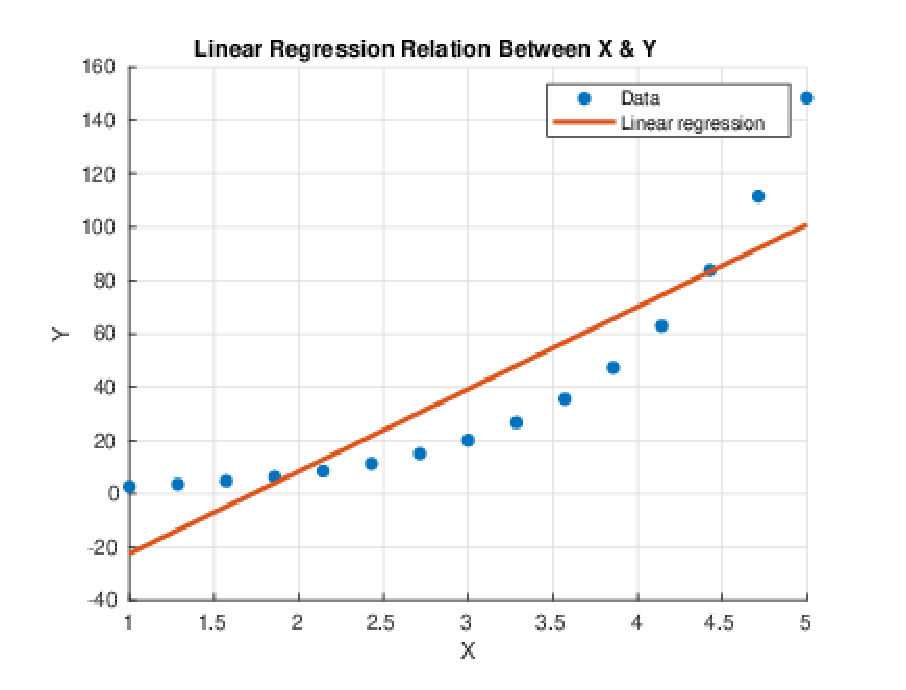
\includegraphics[width=\maxwidth{56.69844455594581em}]{figure_0.eps}
\end{center}

\begin{par}
\begin{flushleft}
As we can see, the model does not fit the data addecuately. We can use a feature mapping and repeat the process with the transformed input:
\end{flushleft}
\end{par}

\begin{matlabcode}
X = feat_map(x)
\end{matlabcode}
\begin{matlaboutput}
X = 15x3    
    1.0000    1.0000    2.7183
    1.0000    1.2857    3.6173
    1.0000    1.5714    4.8135
    1.0000    1.8571    6.4054
    1.0000    2.1429    8.5238
    1.0000    2.4286   11.3427
    1.0000    2.7143   15.0938
    1.0000    3.0000   20.0855
    1.0000    3.2857   26.7281
    1.0000    3.5714   35.5674

\end{matlaboutput}
\begin{matlabcode}

b2 = X\y;
yCalc2 = X*b2;

scatter(x,y,'filled')
hold on 
plot(x,yCalc2,'LineWidth',2)
xlabel('X')
ylabel('Y')
title('Linear Regression Relation Between exp(X) & Y')
legend('Data','Linear regression','Location','north')
grid on
hold off
\end{matlabcode}
\begin{center}
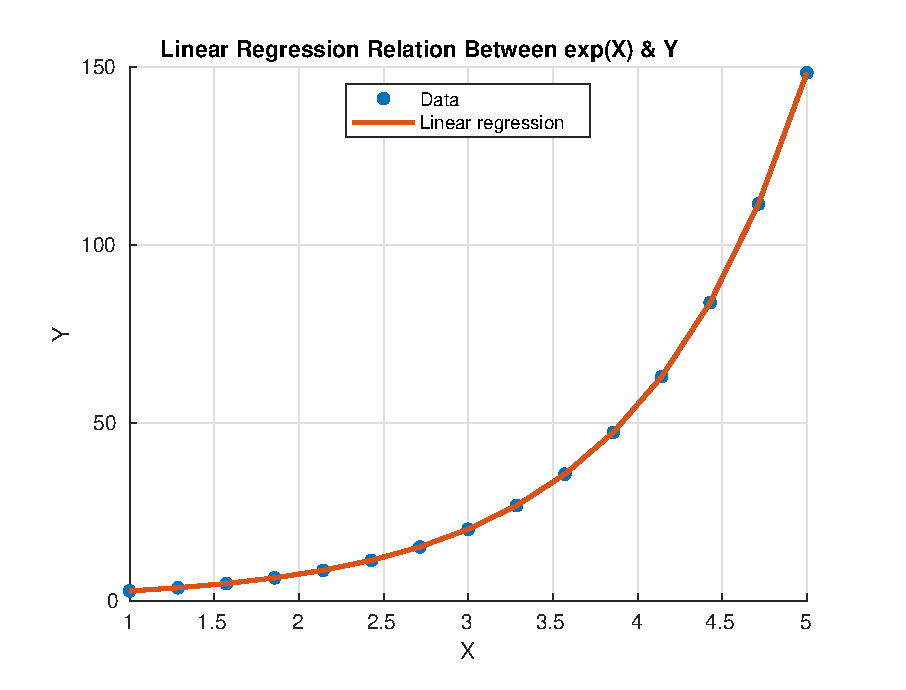
\includegraphics[width=\maxwidth{56.69844455594581em}]{figure_1.eps}
\end{center}

\begin{par}
\begin{flushleft}
As we can see, the model is now perfectly fitting the data!
\end{flushleft}
\end{par}


\begin{matlabcode}
function X=feat_map(x)
    X = [ones(size(x)) x exp(x)];
end
\end{matlabcode}

\end{document}
